\documentclass[11pt,addpoints,answers]{exam}
\usepackage[margin=1in]{geometry}
\usepackage{amsmath, amsfonts}
\usepackage{enumerate}
\usepackage{graphicx}
\usepackage{titling}
\usepackage{url}
\usepackage{xfrac}
\usepackage{geometry}
\usepackage{graphicx}
\usepackage{natbib}
\usepackage{amsmath}
\usepackage{amssymb}
\usepackage{amsthm}
\usepackage{paralist}
\usepackage{epstopdf}
\usepackage{tabularx}
\usepackage{longtable}
\usepackage{multirow}
\usepackage{multicol}
\usepackage[colorlinks=true,urlcolor=blue]{hyperref}
\usepackage{fancyvrb}
\usepackage{algorithm}
\usepackage{algorithmic}
\usepackage{float}
\usepackage{paralist}
\usepackage[svgname]{xcolor}
\usepackage{enumerate}
\usepackage{array}
\usepackage{times}
\usepackage{url}
\usepackage{comment}
\usepackage{environ}
\usepackage{times}
\usepackage{textcomp}
\usepackage{caption}
\usepackage[colorlinks=true,urlcolor=blue]{hyperref}
\usepackage{listings}
\usepackage{parskip} % For NIPS style paragraphs.
\usepackage[compact]{titlesec} % Less whitespace around titles
\usepackage[inline]{enumitem} % For inline enumerate* and itemize*
\usepackage{datetime}
\usepackage{comment}
% \usepackage{minted}
\usepackage{lastpage}
\usepackage{color}
\usepackage{xcolor}
\usepackage{listings}
\usepackage{tikz}
\usetikzlibrary{shapes,decorations,bayesnet}
%\usepackage{framed}
\usepackage{booktabs}
\usepackage{cprotect}
\usepackage{xcolor}
\usepackage{verbatimbox}
\usepackage[many]{tcolorbox}
\usepackage{cancel}
\usepackage{wasysym}
\usepackage{mdframed}
\usepackage{subcaption}
\usetikzlibrary{shapes.geometric}

%%%%%%%%%%%%%%%%%%%%%%%%%%%%%%%%%%%%%%%%%%%
% Formatting for \CorrectChoice of "exam" %
%%%%%%%%%%%%%%%%%%%%%%%%%%%%%%%%%%%%%%%%%%%

\CorrectChoiceEmphasis{}
\checkedchar{\blackcircle}

%%%%%%%%%%%%%%%%%%%%%%%%%%%%%%%%%%%%%%%%%%%
% Better numbering                        %
%%%%%%%%%%%%%%%%%%%%%%%%%%%%%%%%%%%%%%%%%%%

\numberwithin{equation}{section} % Number equations within sections (i.e. 1.1, 1.2, 2.1, 2.2 instead of 1, 2, 3, 4)
\numberwithin{figure}{section} % Number figures within sections (i.e. 1.1, 1.2, 2.1, 2.2 instead of 1, 2, 3, 4)
\numberwithin{table}{section} % Number tables within sections (i.e. 1.1, 1.2, 2.1, 2.2 instead of 1, 2, 3, 4)


%%%%%%%%%%%%%%%%%%%%%%%%%%%%%%%%%%%%%%%%%%%
% Common Math Commands                    %
%%%%%%%%%%%%%%%%%%%%%%%%%%%%%%%%%%%%%%%%%%%

%%%%%%%%%%%%%%%%%%%%%%%%%%%%%%%%%%%%%%%%%%
% Custom commands                        %
%%%%%%%%%%%%%%%%%%%%%%%%%%%%%%%%%%%%%%%%%%

\newcommand{\vc}[1]{\boldsymbol{#1}}
\newcommand{\adj}[1]{\frac{d J}{d #1}}
\newcommand{\chain}[2]{\adj{#2} = \adj{#1}\frac{d #1}{d #2}}

% mathcal
\newcommand{\Ac}{\mathcal{A}}
\newcommand{\Bc}{\mathcal{B}}
\newcommand{\Cc}{\mathcal{C}}
\newcommand{\Dc}{\mathcal{D}}
\newcommand{\Ec}{\mathcal{E}}
\newcommand{\Fc}{\mathcal{F}}
\newcommand{\Gc}{\mathcal{G}}
\newcommand{\Hc}{\mathcal{H}}
\newcommand{\Ic}{\mathcal{I}}
\newcommand{\Jc}{\mathcal{J}}
\newcommand{\Kc}{\mathcal{K}}
\newcommand{\Lc}{\mathcal{L}}
\newcommand{\Mc}{\mathcal{M}}
\newcommand{\Nc}{\mathcal{N}}
\newcommand{\Oc}{\mathcal{O}}
\newcommand{\Pc}{\mathcal{P}}
\newcommand{\Qc}{\mathcal{Q}}
\newcommand{\Rc}{\mathcal{R}}
\newcommand{\Sc}{\mathcal{S}}
\newcommand{\Tc}{\mathcal{T}}
\newcommand{\Uc}{\mathcal{U}}
\newcommand{\Vc}{\mathcal{V}}
\newcommand{\Wc}{\mathcal{W}}
\newcommand{\Xc}{\mathcal{X}}
\newcommand{\Yc}{\mathcal{Y}}
\newcommand{\Zc}{\mathcal{Z}}

% mathbb
\newcommand{\Ab}{\mathbb{A}}
\newcommand{\Bb}{\mathbb{B}}
\newcommand{\Cb}{\mathbb{C}}
\newcommand{\Db}{\mathbb{D}}
\newcommand{\Eb}{\mathbb{E}}
\newcommand{\Fb}{\mathbb{F}}
\newcommand{\Gb}{\mathbb{G}}
\newcommand{\Hb}{\mathbb{H}}
\newcommand{\Ib}{\mathbb{I}}
\newcommand{\Jb}{\mathbb{J}}
\newcommand{\Kb}{\mathbb{K}}
\newcommand{\Lb}{\mathbb{L}}
\newcommand{\Mb}{\mathbb{M}}
\newcommand{\Nb}{\mathbb{N}}
\newcommand{\Ob}{\mathbb{O}}
\newcommand{\Pb}{\mathbb{P}}
\newcommand{\Qb}{\mathbb{Q}}
\newcommand{\Rb}{\mathbb{R}}
\newcommand{\Sb}{\mathbb{S}}
\newcommand{\Tb}{\mathbb{T}}
\newcommand{\Ub}{\mathbb{U}}
\newcommand{\Vb}{\mathbb{V}}
\newcommand{\Wb}{\mathbb{W}}
\newcommand{\Xb}{\mathbb{X}}
\newcommand{\Yb}{\mathbb{Y}}
\newcommand{\Zb}{\mathbb{Z}}

% mathbf lowercase
\newcommand{\av}{\mathbf{a}}
\newcommand{\bv}{\mathbf{b}}
\newcommand{\cv}{\mathbf{c}}
\newcommand{\dv}{\mathbf{d}}
\newcommand{\ev}{\mathbf{e}}
\newcommand{\fv}{\mathbf{f}}
\newcommand{\gv}{\mathbf{g}}
\newcommand{\hv}{\mathbf{h}}
\newcommand{\iv}{\mathbf{i}}
\newcommand{\jv}{\mathbf{j}}
\newcommand{\kv}{\mathbf{k}}
\newcommand{\lv}{\mathbf{l}}
\newcommand{\mv}{\mathbf{m}}
\newcommand{\nv}{\mathbf{n}}
\newcommand{\ov}{\mathbf{o}}
\newcommand{\pv}{\mathbf{p}}
\newcommand{\qv}{\mathbf{q}}
\newcommand{\rv}{\mathbf{r}}
\newcommand{\sv}{\mathbf{s}}
\newcommand{\tv}{\mathbf{t}}
\newcommand{\uv}{\mathbf{u}}
\newcommand{\vv}{\mathbf{v}}
\newcommand{\wv}{\mathbf{w}}
\newcommand{\xv}{\mathbf{x}}
\newcommand{\yv}{\mathbf{y}}
\newcommand{\zv}{\mathbf{z}}

% mathbf uppercase
\newcommand{\Av}{\mathbf{A}}
\newcommand{\Bv}{\mathbf{B}}
\newcommand{\Cv}{\mathbf{C}}
\newcommand{\Dv}{\mathbf{D}}
\newcommand{\Ev}{\mathbf{E}}
\newcommand{\Fv}{\mathbf{F}}
\newcommand{\Gv}{\mathbf{G}}
\newcommand{\Hv}{\mathbf{H}}
\newcommand{\Iv}{\mathbf{I}}
\newcommand{\Jv}{\mathbf{J}}
\newcommand{\Kv}{\mathbf{K}}
\newcommand{\Lv}{\mathbf{L}}
\newcommand{\Mv}{\mathbf{M}}
\newcommand{\Nv}{\mathbf{N}}
\newcommand{\Ov}{\mathbf{O}}
\newcommand{\Pv}{\mathbf{P}}
\newcommand{\Qv}{\mathbf{Q}}
\newcommand{\Rv}{\mathbf{R}}
\newcommand{\Sv}{\mathbf{S}}
\newcommand{\Tv}{\mathbf{T}}
\newcommand{\Uv}{\mathbf{U}}
\newcommand{\Vv}{\mathbf{V}}
\newcommand{\Wv}{\mathbf{W}}
\newcommand{\Xv}{\mathbf{X}}
\newcommand{\Yv}{\mathbf{Y}}
\newcommand{\Zv}{\mathbf{Z}}

% bold greek lowercase
\newcommand{\alphav     }{\boldsymbol \alpha     }
\newcommand{\betav      }{\boldsymbol \beta      }
\newcommand{\gammav     }{\boldsymbol \gamma     }
\newcommand{\deltav     }{\boldsymbol \delta     }
\newcommand{\epsilonv   }{\boldsymbol \epsilon   }
\newcommand{\varepsilonv}{\boldsymbol \varepsilon}
\newcommand{\zetav      }{\boldsymbol \zeta      }
\newcommand{\etav       }{\boldsymbol \eta       }
\newcommand{\thetav     }{\boldsymbol \theta     }
\newcommand{\varthetav  }{\boldsymbol \vartheta  }
\newcommand{\iotav      }{\boldsymbol \iota      }
\newcommand{\kappav     }{\boldsymbol \kappa     }
\newcommand{\varkappav  }{\boldsymbol \varkappa  }
\newcommand{\lambdav    }{\boldsymbol \lambda    }
\newcommand{\muv        }{\boldsymbol \mu        }
\newcommand{\nuv        }{\boldsymbol \nu        }
\newcommand{\xiv        }{\boldsymbol \xi        }
\newcommand{\omicronv   }{\boldsymbol \omicron   }
\newcommand{\piv        }{\boldsymbol \pi        }
\newcommand{\varpiv     }{\boldsymbol \varpi     }
\newcommand{\rhov       }{\boldsymbol \rho       }
\newcommand{\varrhov    }{\boldsymbol \varrho    }
\newcommand{\sigmav     }{\boldsymbol \sigma     }
\newcommand{\varsigmav  }{\boldsymbol \varsigma  }
\newcommand{\tauv       }{\boldsymbol \tau       }
\newcommand{\upsilonv   }{\boldsymbol \upsilon   }
\newcommand{\phiv       }{\boldsymbol \phi       }
\newcommand{\varphiv    }{\boldsymbol \varphi    }
\newcommand{\chiv       }{\boldsymbol \chi       }
\newcommand{\psiv       }{\boldsymbol \psi       }
\newcommand{\omegav     }{\boldsymbol \omega     }

% bold greek uppercase
\newcommand{\Gammav     }{\boldsymbol \Gamma     }
\newcommand{\Deltav     }{\boldsymbol \Delta     }
\newcommand{\Thetav     }{\boldsymbol \Theta     }
\newcommand{\Lambdav    }{\boldsymbol \Lambda    }
\newcommand{\Xiv        }{\boldsymbol \Xi        }
\newcommand{\Piv        }{\boldsymbol \Pi        }
\newcommand{\Sigmav     }{\boldsymbol \Sigma     }
\newcommand{\Upsilonv   }{\boldsymbol \Upsilon   }
\newcommand{\Phiv       }{\boldsymbol \Phi       }
\newcommand{\Psiv       }{\boldsymbol \Psi       }
\newcommand{\Omegav     }{\boldsymbol \Omega     }

%%%%%%%%%%%%%%%%%%%%%%%%%%%%%%%%%%%%%%%%%%%
% Code highlighting with listings         %
%%%%%%%%%%%%%%%%%%%%%%%%%%%%%%%%%%%%%%%%%%%

\definecolor{bluekeywords}{rgb}{0.13,0.13,1}
\definecolor{greencomments}{rgb}{0,0.5,0}
\definecolor{redstrings}{rgb}{0.9,0,0}
\definecolor{light-gray}{gray}{0.95}

\newcommand{\MYhref}[3][blue]{\href{#2}{\color{#1}{#3}}}%

\definecolor{dkgreen}{rgb}{0,0.6,0}
\definecolor{gray}{rgb}{0.5,0.5,0.5}
\definecolor{mauve}{rgb}{0.58,0,0.82}

\lstdefinelanguage{Shell}{
  keywords={tar, cd, make},
  %keywordstyle=\color{bluekeywords}\bfseries,
  alsoletter={+},
  ndkeywords={python, py, javac, java, gcc, c, g++, cpp, .txt, octave, m, .tar},
  %ndkeywordstyle=\color{bluekeywords}\bfseries,
  identifierstyle=\color{black},
  sensitive=false,
  comment=[l]{//},
  morecomment=[s]{/*}{*/},
  commentstyle=\color{purple}\ttfamily,
  stringstyle=\color{red}\ttfamily,
  morestring=[b]',
  morestring=[b]",
  backgroundcolor = \color{light-gray}
}

\lstset{columns=fixed, basicstyle=\ttfamily,
    backgroundcolor=\color{light-gray},xleftmargin=0.5cm,frame=tlbr,framesep=4pt,framerule=0pt}



%%%%%%%%%%%%%%%%%%%%%%%%%%%%%%%%%%%%%%%%%%%
% Custom box for highlights               %
%%%%%%%%%%%%%%%%%%%%%%%%%%%%%%%%%%%%%%%%%%%

% Define box and box title style
\tikzstyle{mybox} = [fill=blue!10, very thick,
    rectangle, rounded corners, inner sep=1em, inner ysep=1em]

% \newcommand{\notebox}[1]{
% \begin{tikzpicture}
% \node [mybox] (box){%
%     \begin{minipage}{\textwidth}
%     #1
%     \end{minipage}
% };
% \end{tikzpicture}%
% }

\NewEnviron{notebox}{
\begin{tikzpicture}
\node [mybox] (box){
    \begin{minipage}{\textwidth}
        \BODY
    \end{minipage}
};
\end{tikzpicture}
}

%%%%%%%%%%%%%%%%%%%%%%%%%%%%%%%%%%%%%%%%%%%
% Commands showing / hiding solutions     %
%%%%%%%%%%%%%%%%%%%%%%%%%%%%%%%%%%%%%%%%%%%

%% To HIDE SOLUTIONS (to post at the website for students), set this value to 0: \def\issoln{0}
\def\issoln{0}
% Some commands to allow solutions to be embedded in the assignment file.
\ifcsname issoln\endcsname \else \def\issoln{0} \fi
% Default to an empty solutions environ.
\NewEnviron{soln}{}{}
% Default to an empty qauthor environ.
\NewEnviron{qauthor}{}{}
% Default to visible (but empty) solution box.
\newtcolorbox[]{studentsolution}[1][]{%
    breakable,
    enhanced,
    colback=white,
    title=Solution,
    #1
}

\if\issoln 1
% Otherwise, include solutions as below.
\RenewEnviron{soln}{
    \leavevmode\color{red}\ignorespaces
    \textbf{Solution} \BODY
}{}
\fi

\if\issoln 1
% Otherwise, include solutions as below.
\RenewEnviron{solution}{}
\fi

%%%%%%%%%%%%%%%%%%%%%%%%%%%%%%%%%%%%%%%%%%%
% Commands for customizing the assignment %
%%%%%%%%%%%%%%%%%%%%%%%%%%%%%%%%%%%%%%%%%%%

\newcommand{\courseNum}{\href{https://geometric3d.github.io}{16822}}
\newcommand{\courseName}{\href{https://geometric3d.github.io}{Geometry-based Methods in Vision}}
\newcommand{\courseSem}{\href{https://geometric3d.github.io}{Fall 2022}}
\newcommand{\courseUrl}{\url{https://piazza.com/cmu/fall2022/16822}}
\newcommand{\hwNum}{Problem Set 2}
\newcommand{\hwTopic}{Projective Geometry and Homography }
\newcommand{\hwName}{\hwNum: \hwTopic}
\newcommand{\outDate}{Sep. 20, 2022}
\newcommand{\dueDate}{Sep. 27, 2022 11:59 PM}
\newcommand{\instructorName}{Shubham Tulsiani}
\newcommand{\taNames}{Mosam Dabhi, Kangle Deng, Jenny Nan}

%\pagestyle{fancyplain}
\lhead{\hwName}
\rhead{\courseNum}
\cfoot{\thepage{} of \numpages{}}

\title{\textsc{\hwName}} % Title


\author{}

\date{}

%%%%%%%%%%%%%%%%%%%%%%%%%%%%%%%%%%%%%%%%%%%%%%%%%
% Useful commands for typesetting the questions %
%%%%%%%%%%%%%%%%%%%%%%%%%%%%%%%%%%%%%%%%%%%%%%%%%

\newcommand \expect {\mathbb{E}}
\newcommand \mle [1]{{\hat #1}^{\rm MLE}}
\newcommand \map [1]{{\hat #1}^{\rm MAP}}
\newcommand \argmax {\operatorname*{argmax}}
\newcommand \argmin {\operatorname*{argmin}}
\newcommand \code [1]{{\tt #1}}
\newcommand \datacount [1]{\#\{#1\}}
\newcommand \ind [1]{\mathbb{I}\{#1\}}

\newcommand{\blackcircle}{\tikz\draw[black,fill=black] (0,0) circle (1ex);}
\renewcommand{\circle}{\tikz\draw[black] (0,0) circle (1ex);}

\newcommand{\pts}[1]{\textbf{[#1 pts]}}

%%%%%%%%%%%%%%%%%%%%%%%%%%
% Document configuration %
%%%%%%%%%%%%%%%%%%%%%%%%%%

% Don't display a date in the title and remove the white space
\predate{}
\postdate{}
\date{}

%%%%%%%%%%%%%%%%%%
% Begin Document %
%%%%%%%%%%%%%%%%%%


\begin{document}

\section*{}
\begin{center}
  \textsc{\LARGE \hwNum} \\
%   \textsc{\LARGE \hwTopic\footnote{Compiled on \today{} at \currenttime{}}} \\
  \vspace{1em}
  \textsc{\large \courseNum{} \courseName{} (\courseSem)} \\
  %\vspace{0.25em}
  \courseUrl\\
  \vspace{1em}
  OUT: \outDate \\
  DUE: \dueDate \\
  Instructor: \instructorName \\
  TAs: \taNames
\end{center}

\section*{START HERE: Instructions}
\begin{itemize}
\item \textbf{Collaboration policy:} All are encouraged to work together BUT you must do your own work (code and write up). If you work with someone, please include their name in your write up and cite any code that has been discussed. If we find highly identical write-ups or code without proper accreditation of collaborators, we will take action according to university policies, i.e. you will likely fail the course. See the \href{https://www.dropbox.com/s/z6o0tinc9eaez46/L01_Overview.pdf?dl=0}{Academic Integrity Section} detailed in the initial lecture for more information.

\item\textbf{Late Submission Policy:} There are \textbf{no} late days for Problem Set submissions.

\item\textbf{Submitting your work:}

\begin{itemize}

\item We will be using Gradescope (\url{https://gradescope.com/}) to submit the Problem Sets. Please use the provided template. Submissions can be written in LaTeX. Regrade requests can be made, however this gives the TA the opportunity to regrade your entire paper, meaning if additional mistakes are found then points will be deducted.
Each derivation/proof should be  completed on a separate page. For short answer questions you \textbf{should} include your work in your solution.  
\end{itemize}

\item \textbf{Materials:} The data that you will need in order to complete this assignment is posted along with the writeup and template on Piazza.

\end{itemize}

For multiple choice or select all that apply questions, replace \lstinline{\choice} with \lstinline{\CorrectChoice} to obtain a shaded box/circle, and don't change anything else.

\clearpage

\section*{Instructions for Specific Problem Types}

For ``Select One" questions, please fill in the appropriate bubble completely:

\begin{quote}
\textbf{Select One:} Who taught this course?
     \begin{checkboxes}
     \CorrectChoice Shubham Tulsiani
     \choice Deepak Pathak
     \choice Fernando De la Torre
     \choice Deva Ramanan
    \end{checkboxes}
\end{quote}

For ``Select all that apply" questions, please fill in all appropriate squares completely:

\begin{quote}
\textbf{Select all that apply:} Which are scientists?
{
    \checkboxchar{$\Box$} \checkedchar{$\blacksquare$}
    \begin{checkboxes}
     \CorrectChoice Stephen Hawking
     \CorrectChoice Albert Einstein
     \CorrectChoice Isaac Newton
     \choice None of the above
    \end{checkboxes}
    }
\end{quote}

For questions where you must fill in a blank, please make sure your final answer is fully included in the given space. You may cross out answers or parts of answers, but the final answer must still be within the given space.

\begin{quote}
\textbf{Fill in the blank:} What is the course number?

\begin{tcolorbox}[fit,height=1cm, width=4cm, blank, borderline={1pt}{-2pt},nobeforeafter, halign=center, valign=center]
    \begin{center}\huge16-822\end{center}
    \end{tcolorbox}\hspace{2cm}
\end{quote}

\clearpage

\section{2D Projective Geometry  [18 pts]}
\begin{questions}

\question (a) \textbf{[2 pts]} Calculate the line passing through 2 given points: (1) $\pv_1= [3,4,1]^T, \pv_2 = [4,3,0]^T$, (2) $\pv_1= [3,4,2022]^T, \pv_2 = [3,4,-1967]^T$.

(b) \textbf{[2 pts]} Calculate the intersection point between 2 given lines: (1) $\lv_1 = [3,4,1]^T, \lv_2 = [0,0,1]^T $, (2) $\lv_1= [3,4,1]^T, \lv_2 = [3,4,2]^T$.

\begin{tcolorbox}[fit,height=5cm, width=\textwidth, blank, borderline={0.5pt}{-2pt},halign=left, valign=center, nobeforeafter]


\end{tcolorbox}

\question \textbf{[3 pts]} Suppose a conic in 2D projective space is given by $\Cv = \lv\mv^T + \mv\lv^T$, where $\lv$ and $\mv$ are 2 lines. Show that a point belongs to $\Cv$ if and only if it is on $\mv$ or $\lv$.

\begin{tcolorbox}[fit,height=5cm, width=\textwidth, blank, borderline={0.5pt}{-2pt},halign=left, valign=center, nobeforeafter]

\end{tcolorbox}

\question \textbf{[4 pts]} Given a transformation $\Hv = \begin{bmatrix}
                 3 & 0 & 0  \\
                 0 & 2 & 0  \\
                 0 & 0 & 1  \\
                \end{bmatrix}$,

(a) transform a point $\pv = [3,4,1]^T$,

(b) transform a line $\lv = [-4, 3, 0]$

(c) transform a conic $\Cv = \begin{bmatrix}
                 1 & 0 & 0  \\
                 0 & 2 & 0  \\
                 0 & 0 & 3  \\
                \end{bmatrix}$

(d) does this transformation leaves the circular points at infinity unchanged? Explain the reason without calculation.

\begin{tcolorbox}[fit,height=5cm, width=\textwidth, blank, borderline={0.5pt}{-2pt},halign=left, valign=center, nobeforeafter]


\end{tcolorbox}

\question \textbf{[4 pts]} Are these 2D projective transformations?

(a) Reflection along a line,

(b) Doubling spherical coordinates: $(r,\theta) \rightarrow (2r, 2\theta)$,

(c) A picture hanging on a wall and its image taken by a camera,

(d) Transformation between these 2 world maps.
\begin{figure}[h!]
    \centering
    \begin{subfigure}{0.48\linewidth}
        \centering
        {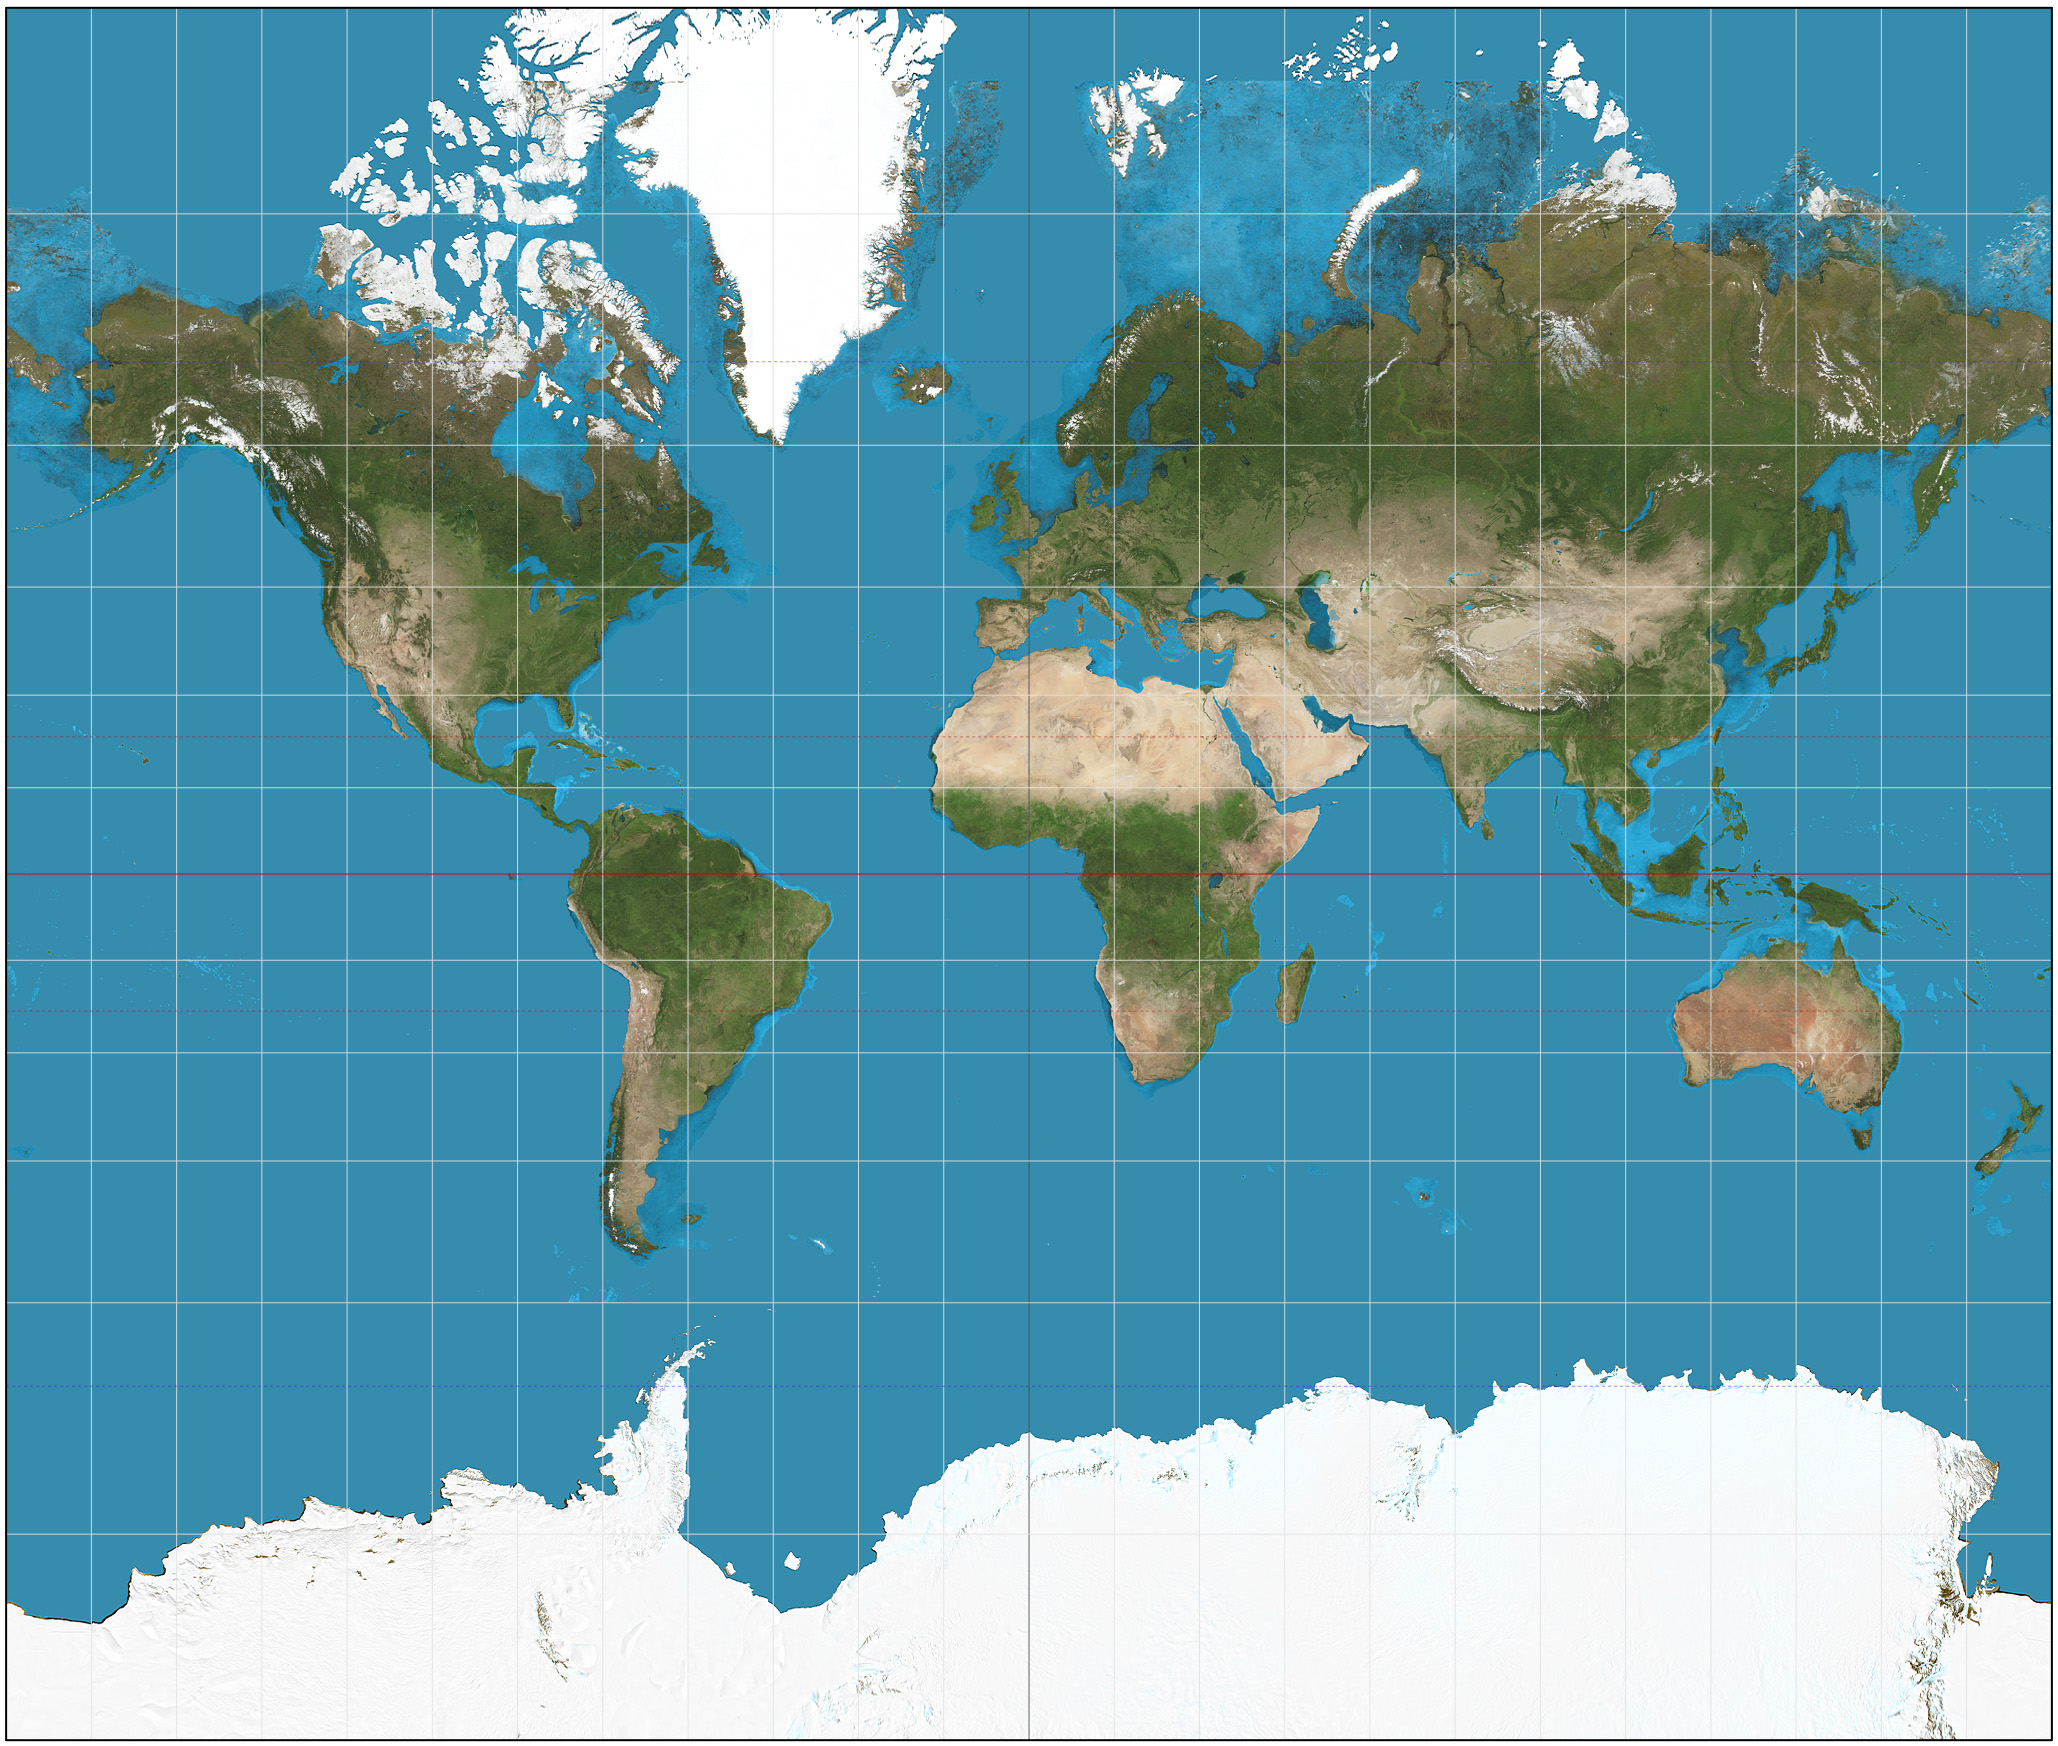
\includegraphics[width=0.33\linewidth]{figures/Mercator_projection_SW.jpg}}
    \end{subfigure}
    \begin{subfigure}{0.48\linewidth}
        \centering
        {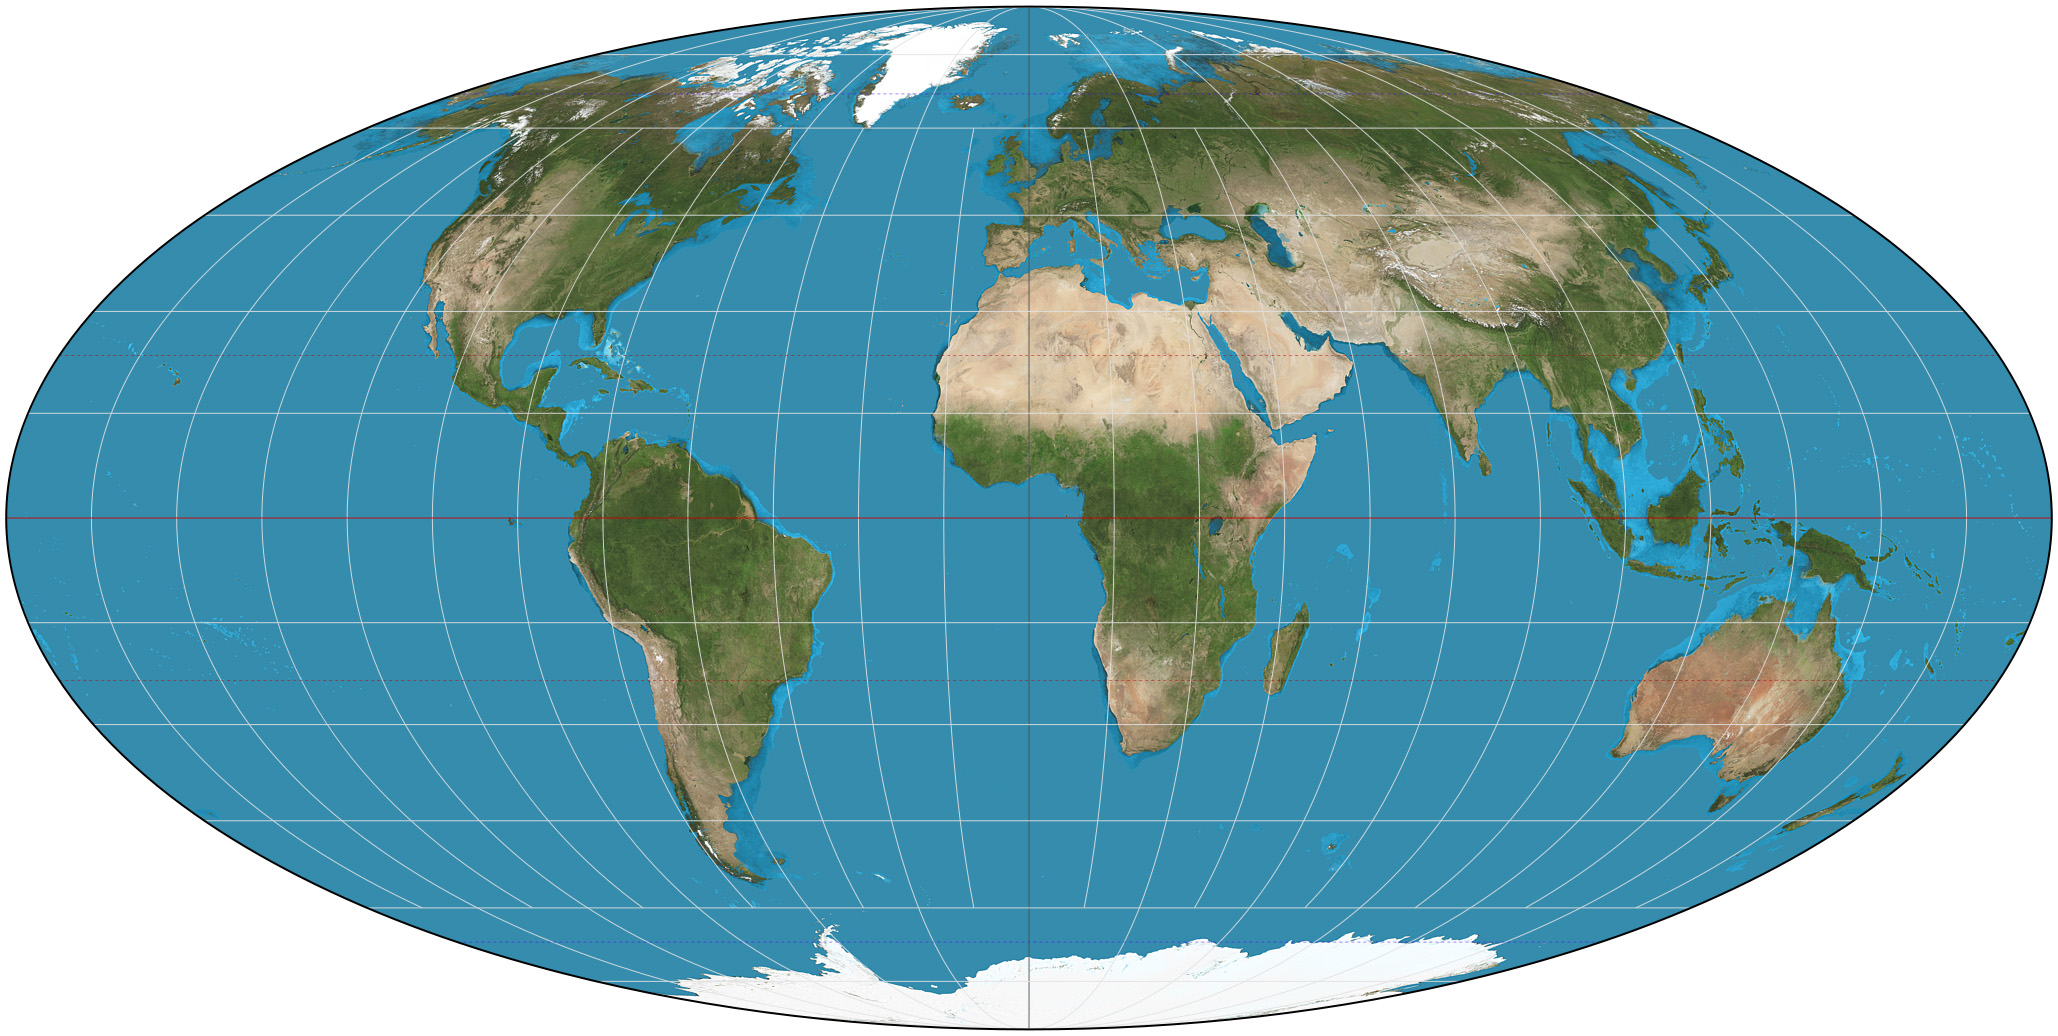
\includegraphics[width=0.5\textwidth]{figures/Mollweide_projection_SW.jpg}}
    \end{subfigure}
\end{figure}

\begin{tcolorbox}[fit,height=5cm, width=\textwidth, blank, borderline={0.5pt}{-2pt},halign=left, valign=center, nobeforeafter]


\end{tcolorbox}

\question \textbf{[3 pts]} Are these statements true or false?


(a) Given a line $\lv$, if both $\Hv_A$ and $\Hv_B$ map $\lv$ to $[0,0,1]^T$, then $\Hv_A\Hv_B^{-1}$ is an affine transformation. 

(b) Instead of annotating orthogonal lines, if we annotate multiple pairs of lines that form 45 degree angles in the metric space, we can still calculate $\Cv_\infty^{\star}{}'$.

(c) If we are allowed to annotate pairs of parallel and orthogonal lines, we need at least 5 pairs of them to calculate $\Cv_\infty^{\star}{}'$.

\begin{tcolorbox}[fit,height=5cm, width=\textwidth, blank, borderline={0.5pt}{-2pt},halign=left, valign=center, nobeforeafter]



\end{tcolorbox}


\section{3D Projective Geometry [12 pts]}

\question \textbf{[3 pts]} Show that the Plucker Representation of a 3D line $\Lv = \xv_1\xv_2^T - \xv_2\xv_1^T$ is equivalent to representing the line as $(\tilde \dv, \tilde \xv \times \tilde \dv)$, i.e. show they have the same elements up to scale.

Notations: $\tilde\dv$ is the unit direction vector along the line, and $\tilde \xv$ is any point on the line. Note that $\tilde\xv$ and $\tilde\dv$ are 3-dim Euclidean coordinates while $\xv_1$ and $\xv_2$ are 4-dim homogeneous coordinates.

\begin{tcolorbox}[fit,height=10cm, width=\textwidth, blank, borderline={0.5pt}{-2pt},halign=left, valign=center, nobeforeafter]


\end{tcolorbox}

\question \textbf{[2 pts]} Suppose $\Uv$ is a $4\times 4$ matrix. $\Uv_{4 \times 4} = [\uv_1, \uv_2, \uv_3, \uv_4]$ and $\Uv^T\Uv = \Iv$.

(a) Suppose $\uv_1, \uv_2, \uv_3$ represent 3 points in the 3D space. What is the plane passing through these 3 points?

(b) Suppose $\uv_1, \uv_2, \uv_3, \uv_4$ represent 4 points in the 3D space. Let $\lv_1$ be the line passing through $\uv_1, \uv_2$, and $\lv_2$ be the line passing through $\uv_3, \uv_4$. Do $\lv_1$ and $\lv_2$ intersect or not? (Only consider real-number points.)

\begin{tcolorbox}[fit,height=5cm, width=\textwidth, blank, borderline={0.5pt}{-2pt},halign=left, valign=center, nobeforeafter]



\end{tcolorbox}

\question \textbf{[4 pts]} (a) Calculate the 3D transformation $\Hv$ that represents the projection onto a plane $\pi = [\nv^T, 0]^T$, where $\nv = [a,b,c]^T$ is a unit vector.

(b) Calculate the 3D transformation $\Hv$ that represents the reflection along a plane $\pi = [\nv^T, 0]^T$, where $\nv = [a,b,c]^T$ is a unit vector.

\begin{tcolorbox}[fit,height=15cm, width=\textwidth, blank, borderline={0.5pt}{-2pt},halign=left, valign=center, nobeforeafter]



\end{tcolorbox}

\question \textbf{[3 pts]} In the lecture, we introduced an algorithm to compute homography between images from 4 pairs of point correspondences. Design an algorithm that instead uses pairs of line correspondences. Write the constraints provided by each correspondence, and how to compute the $\Hv$ that satisfies these.

\begin{tcolorbox}[fit,height=5cm, width=\textwidth, blank, borderline={0.5pt}{-2pt},halign=left, valign=center, nobeforeafter]



\end{tcolorbox}


\end{questions}

\clearpage

\textbf{Collaboration Questions} Please answer the following:

\begin{enumerate}
    \item Did you receive any help whatsoever from anyone in solving this assignment?
    \begin{checkboxes}
     \choice Yes
     \choice No
    \end{checkboxes}
    \begin{itemize}
        \item If you answered `Yes', give full details:
        \item (e.g. “Jane Doe explained to me what is asked in Question 3.4”)
    \end{itemize}

    \begin{tcolorbox}[fit,height=3cm,blank, borderline={1pt}{-2pt},nobeforeafter]
    %Input your solution here.  Do not change any of the specifications of this solution box.
    \end{tcolorbox}

    \item Did you give any help whatsoever to anyone in solving this assignment?
    \begin{checkboxes}
     \choice Yes
     \choice No
    \end{checkboxes}
    \begin{itemize}
        \item If you answered `Yes', give full details:
        \item (e.g. “I pointed Joe Smith to section 2.3 since he didn’t know how to proceed with Question 2”)
    \end{itemize}

    \begin{tcolorbox}[fit,height=3cm,blank, borderline={1pt}{-2pt},nobeforeafter]
    %Input your solution here.  Do not change any of the specifications of this solution box.
    \end{tcolorbox}

    \item Did you find or come across code that implements any part of this assignment ? 
    \begin{checkboxes}
     \choice Yes
     \choice No
    \end{checkboxes}
    \begin{itemize}
        \item If you answered `Yes', give full details: \underline{No}
        \item (book \& page, URL \& location within the page, etc.).
    \end{itemize}
    \begin{tcolorbox}[fit,height=3cm,blank, borderline={1pt}{-2pt},nobeforeafter]
    %Input your solution here.  Do not change any of the specifications of this solution box.
    \end{tcolorbox}
\end{enumerate}

\end{document}